
\begin{figure}[H]
  \centering
  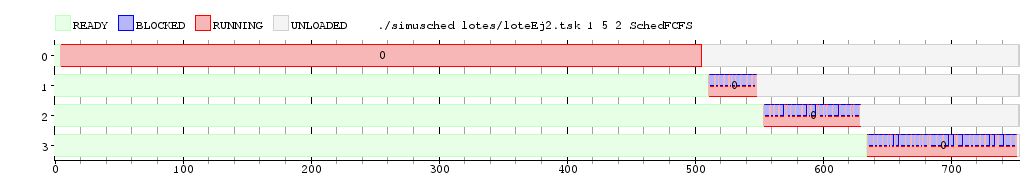
\includegraphics[width=1\textwidth]{img/imgEj2-1}
  \caption{}
  \label{fig:ej2-1}
\end{figure}

\begin{figure}[H]
  \centering
  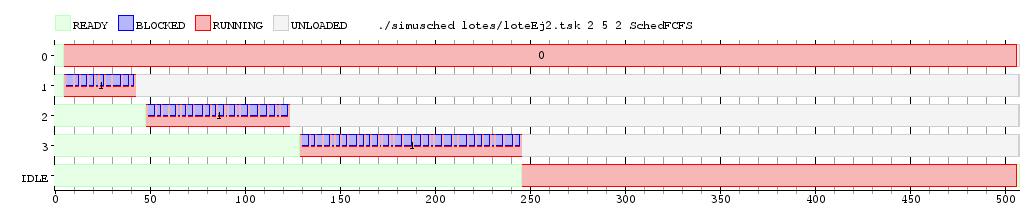
\includegraphics[width=1\textwidth]{img/imgEj2-2}
  \caption{}
  \label{fig:ej2-2}
\end{figure}

\begin{figure}[H]
  \centering
  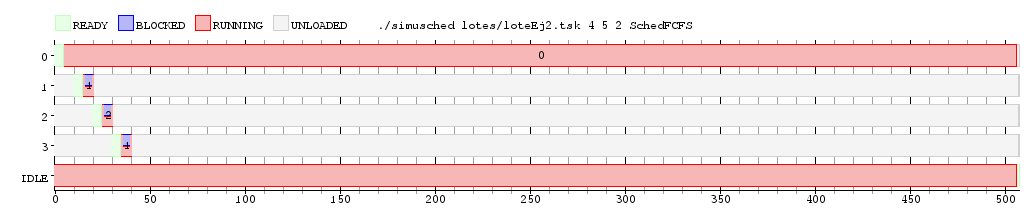
\includegraphics[width=1\textwidth]{img/imgEj2-3}
  \caption{}
  \label{fig:ej2-3}
\end{figure}

\begin{table}[H]
  \center
  \begin{center}
  \begin{tabular}{c|c|c|c|}
    \cline{2-4}
    & \multicolumn{3}{|c|}{\cellcolor{LightCyan}Latencia} \\
    \hline
    \rowcolor{LightCyan}
    \multicolumn{1}{|c|}{\#Procesadores} & 1 & 2 & 4 \\
    \hline
    \multicolumn{1}{|c|}{\cellcolor{LightCyan}Tarea 0} & 5 & 5 & 5 \\
    \multicolumn{1}{|c|}{\cellcolor{LightCyan}Tarea 1} & 501 & 5 & 5 \\
    \multicolumn{1}{|c|}{\cellcolor{LightCyan}Tarea 2} & 502 & 6 & 5 \\
    \multicolumn{1}{|c|}{\cellcolor{LightCyan}Tarea 3} & 502 & 7 & 5 \\
    \hline
    \multicolumn{1}{|c|}{\cellcolor{LightCyan}Promedio} & 377.5 & 5.75 & 5 \\
    \hline
  \end{tabular}
  \end{center}
  \caption{\footnotesize Latencia de cada tarea y latencia promedio según la cantidad de procesadores utilizados.}
  \label{tab:ej2}
\end{table}

Viendo la tabla \ref{tab:ej2} resulta clara la principal desventaja de mantener esta política de \emph{scheduling} con un solo procesador: la latencia de los procesos interactivos resulta altísima debido a que deben esperar a que termine el proceso intensivo en CPU, a pesar de que ellas mismas a penas necesitan utilizarlo. Una diferencia de tiempo tan grande entre que las tres tareas se cargan y efectivamente responden (como puede apreciarse en la figura \ref{fig:ej2-1}) genera para los usuarios la sensación de que ``la máquina se colgó''. De hecho cabe la posibilidad de que si un usuario le pidió alguna información al sistema como parte de un protocolo, al momento de recibirlo esta deje de ser útil o válida.   

Como contrapartida, vemos que el tener 4 procesadores no aporta grandes ventajas sobre tener 2, pues las diferencias de latencia son marginales como puede verse en la tabla, y de hecho uno de los procesadores se desperdicia completamente realizando la tarea \emph{idle} como se aprecia en la figura \ref{fig:ej2-3}.
 


